\chapter{フーリエ双対性、運動量、自由粒子の運動}

\section{基礎から例へ}

量子もつれは量子力学の核心に属するが、その基礎は今や十分に明らかにされたので、それを使い始めることができる。これまでの講義は、意図的に小さな系に依拠してきた。スピン、回転可能な装置、有限個の結果のリスト、そして確率を推測するための繰り返し測定である。これらの実験は、量子力学が発見された歴史的な道筋よりも論理的に単純であるが、最小限の操作的な要素を含んでいる。

\begin{classroomqa}
\audiencequestion{量子力学において、ニュートンの少数の経験的な出発点の役割を果たすものは何か。}
\lecturerresponse{最小の模型は回転可能なスピン装置である。スピンを準備し、軸を選び、測定制御を押し、\(+1\) または \(-1\) を記録し、結果の頻度が分かるまで実験を繰り返す。ベクトル空間、観測量、振幅、ボルンの規則がそれらの統計を整理する。歴史的には、この理論ははるかに豊富な原子現象の集まりから生じたが、論理的にはこの2結果の実験でその構造を明らかにするのに十分である。}
\end{classroomqa}

\begin{classroomqa}
\audiencequestion{スピンや運動量のような各物理量について、同じ統計的手続きを行わなければならないのか。}
\lecturerresponse{はい。観測量は実験配置のクラスと可能な結果に結びついている。形式論は状態と観測量が指定されれば分布を予測するが、観測量の物理的意味はそれがどのように測定されるかによって支えられている。}
\end{classroomqa}

量子もつれを離れる前に、前の議論からの一つの問いに完全な答えを与える価値がある。一重項と三重項のセクターをもつ2つの電子を考え、放射場を別の量子サブシステムとして含める。放射場には真空状態 \(\ket{0_\gamma}\) と1光子状態 \(\ket{1_\gamma}\) がある。粒子数そのものが重ね合わせられてよい。重ね合わせを固定された粒子数の異なる状態に限る規則はない。

授業で議論した理想化された遷移について、最初はもつれていない電子状態は一重項成分と三重項成分の重ね合わせとして書ける。
\begin{equation}
\ket{\uparrow\downarrow}
=
\frac{1}{\sqrt{2}}
\left(\ket{S}+\ket{T_0}\right).
\end{equation}
最初に光子が存在しないとき、状態は
\begin{equation}
\ket{\Psi(0)}
=
\frac{1}{\sqrt{2}}
\left(\ket{S}+\ket{T_0}\right)
\otimes\ket{0_\gamma}.
\label{eq:l9-initial-radiative-state}
\end{equation}
である。一重項成分は放出なしに一重項のままであり、励起された三重項成分は一重項へ緩和して光子を放出できる。
\begin{align}
\ket{S}\ket{0_\gamma}
&\longrightarrow
\ket{S}\ket{0_\gamma}, \\
\ket{T_0}\ket{0_\gamma}
&\longrightarrow
\ket{S}\ket{1_\gamma}.
\end{align}
すると線形性により
\begin{equation}
\ket{\Psi_{\mathrm{final}}}
=
\ket{S}\otimes
\frac{\ket{0_\gamma}+\ket{1_\gamma}}{\sqrt{2}}.
\label{eq:l9-final-radiative-state}
\end{equation}
が得られる。

\begin{figure}[htbp]
\centering
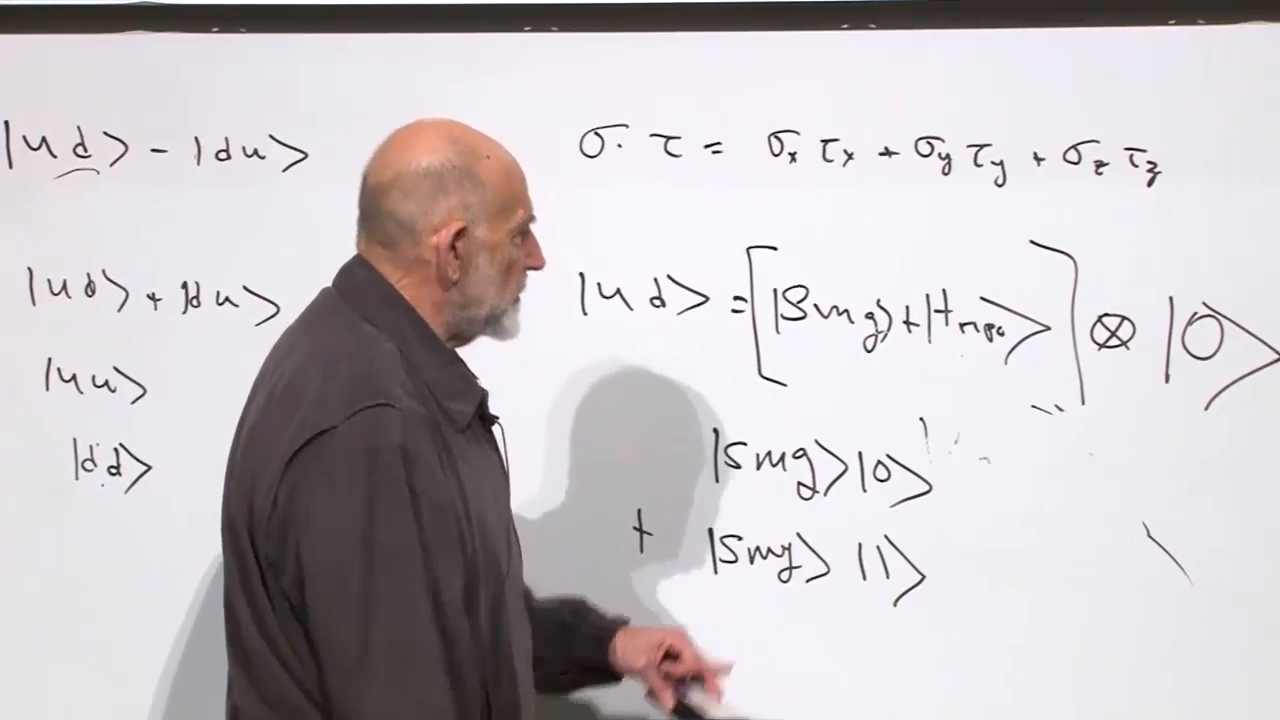
\includegraphics[width=0.88\textwidth]{lecture_09_figure_01.png}
\caption{電子状態は一重項成分と三重項成分に分解され、放射緩和の前に光子真空とテンソル積をとられる。}
\lectureframe{00:05:10}
\end{figure}

最終的な表式は電子対と放射場の間の積である。\(\ket{S}\) がもつれているので2つの電子は互いにもつれているが、放射場は0光子と1光子の重ね合わせに置かれる。この例が微妙なのは、相互作用がもつれを再分配したからである。初期の電子の積状態はもつれた電子対へ発展するが、最終的な理想化された電子-放射状態は因子化する。

\begin{classroomqa}
\audiencequestion{入射光子があれば遷移を逆転させ、電子のもつれを解くことができるか。}
\lecturerresponse{いいえ。時間反転した過程には、適切な光子状態、モード、位相、エネルギー、そして相互作用の履歴が必要である。放出された光子を反射して戻すことは、閉じた系全体の逆の時間発展を整えることの略記であり、任意の光子がもつれを解消すると主張することではなかった。}
\end{classroomqa}

\begin{classroomqa}
\audiencequestion{外部磁場が導入されていないのに、なぜ三重項は放出するのか。}
\lecturerresponse{電子は互いに、そして量子化された電磁場と相互作用する。スピンに依存する相互作用により一方のスピン配置がエネルギー的に有利になり、余分なエネルギーは放射として出て行くことができる。外部の測定装置は必要ない。これは結合した電子と場の通常のユニタリーダイナミクスである。}
\end{classroomqa}

その残った点が片づいたので、ここでスピンを忘れ、最も単純な運動の問題、すなわち一次元直線上の1粒子を研究する。

\section{平面波とフーリエ対}

物理学に戻る前に、数学的な間奏が必要である。次から始めよう。
\begin{equation}
e^{ipx}=\cos(px)+i\sin(px).
\end{equation}
この段階では \(p\) は単に振動の速さを制御する実数である。この表式には時間依存性がなく、したがってまだ動く波を記述していない。\(x\) の関数として見慣れた正弦波の形をとるので、平面波と呼ばれる。

十分に正則な関数のある広いクラスは、そのようなモードに分解できる。以下では、下の積分に対して十分に良い振る舞いをする関数のみを考える。すなわち、空間的無限遠で発散してはならず、後の物理的な波動関数は二乗可積分である。対称な規格化の慣習を採用すると、フーリエ変換対は
\begin{align}
\psi(x)
&=
\int_{-\infty}^{\infty}
\frac{dp}{\sqrt{2\pi}}\,
\widetilde{\psi}(p)e^{ipx},
\label{eq:l9-fourier-forward}\\
\widetilde{\psi}(p)
&=
\int_{-\infty}^{\infty}
\frac{dx}{\sqrt{2\pi}}\,
\psi(x)e^{-ipx}.
\label{eq:l9-fourier-inverse}
\end{align}
となる。係数\(\widetilde{\psi}(p)\)は、フーリエラベル\(p\)をもつモードの複素振幅である。\(1/\sqrt{2\pi}\)の因子は慣習的なものであり、各方向に1つずつ置くことで2つの式が互いに逆の形に見える。指数における相対的な負符号は本質的である。

\begin{figure}[htbp]
\centering
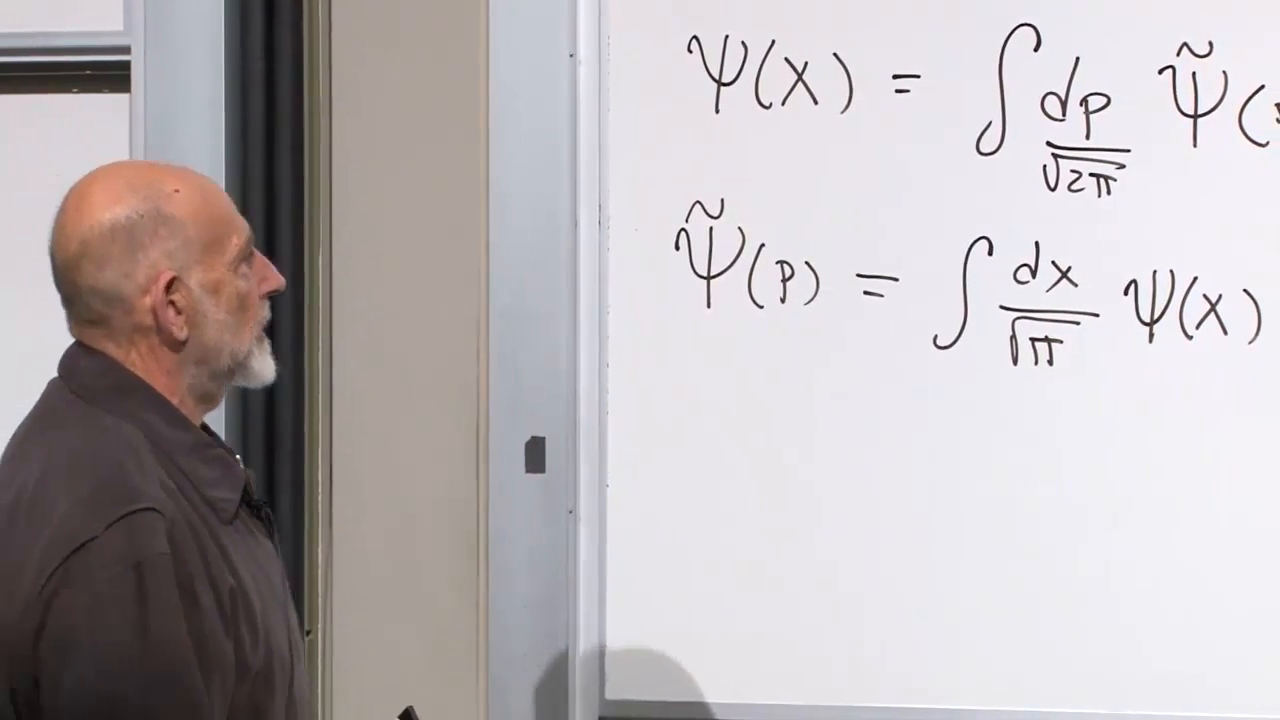
\includegraphics[width=0.88\textwidth]{lecture_09_figure_02.png}
\caption{対称なフーリエ変換対：関数は平面波に分解され、モード振幅は逆変換によって復元される。}
\lectureframe{00:14:35}
\end{figure}

\begin{classroomqa}
\audiencequestion{\(\psi(x)\)と\(\widetilde{\psi}(p)\)は複素数であることを意図しているのか。}
\lecturerresponse{一般には、その通りである。特殊な関数がたまたま実数であることもあり、その場合にはそのフーリエ係数は追加の複素共役関係を満たすが、量子振幅は自然に複素数であり、ここでは実数性の制限は課されない。}
\end{classroomqa}

\begin{classroomqa}
\audiencequestion{なぜ\(2\pi\)をすべて一方の変換に置くのではなく、対称な因子\(1/\sqrt{2\pi}\)を用いるのか。}
\lecturerresponse{どちらの慣習も整合的である。対称な選択では、順変換と逆変換は指数の符号だけが異なる。物理的予測は、関連するすべての規格化を整合的に変更する限り、慣習に依存しない。}
\end{classroomqa}

\(x\)と\(p\)の間の相互関係はすでに見えている。一方の関数は、他方の変数について積分することによって分解される。今のところこれはフーリエ解析である。まもなく同じ対が位置と運動量になる。

\section{操作としてのディラックのデルタ}

直感的なデルタ関数は、幅がゼロに近づき、高さが発散し、面積が1であるスパイクである。この描像は有用だが、操作的定義の方がより信頼できる。適切な任意のテスト関数\(f\)に対して、
\begin{equation}
\int_{-\infty}^{\infty}
dx\,\delta(x-x')f(x)
=f(x').
\label{eq:l9-delta-sampling}
\end{equation}
三つのよく知られた規則が同じ考えを表している。
\begin{align}
f(x)\delta(x-x')
&=
f(x')\delta(x-x'),
\label{eq:l9-delta-multiplication}\\
\int_{-\infty}^{\infty}dx\,\delta(x-x')
&=1,
\label{eq:l9-delta-area}\\
\int_{-\infty}^{\infty}dx\,\delta(x-x')f(x)
&=f(x').
\end{align}
第一の規則が成り立つのは、デルタが\(x=x'\)のところにのみ台をもつからである。第二の規則では、スパイクを平行移動してもその位置が変わるだけで面積は変わらない。これら二つの規則を組み合わせると第三の規則が得られる。

\begin{figure}[htbp]
\centering
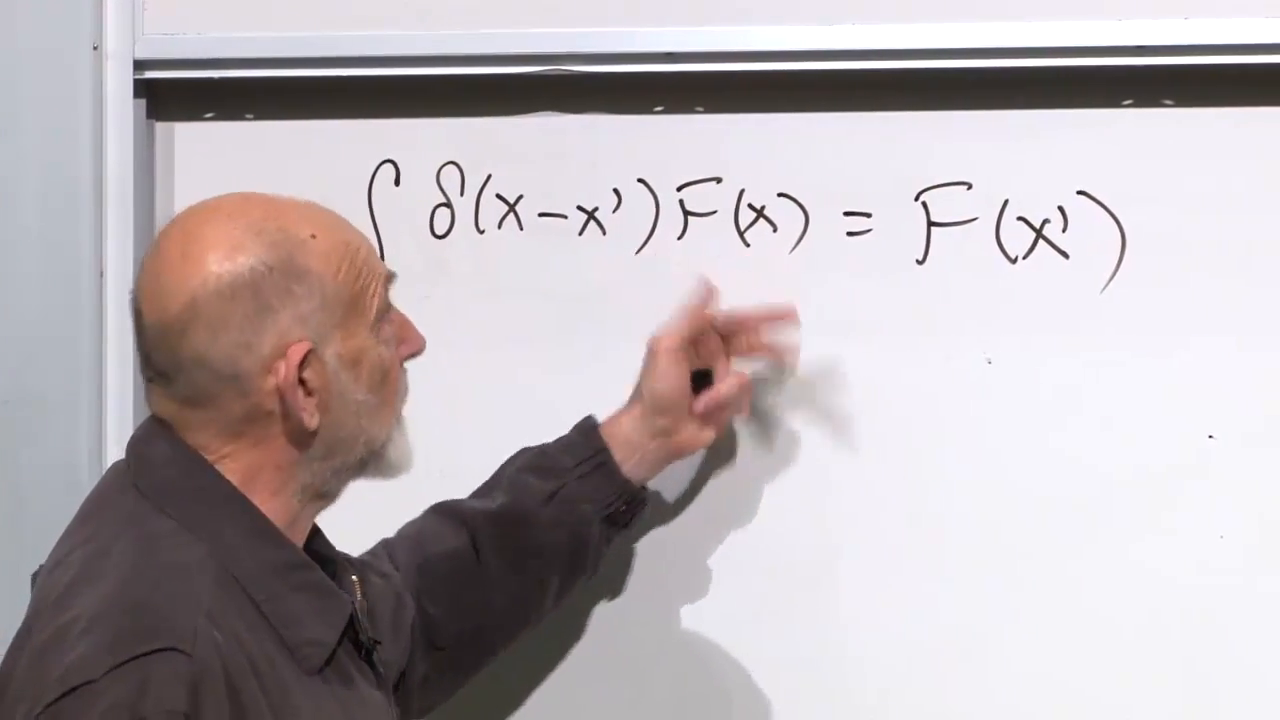
\includegraphics[width=0.88\textwidth]{lecture_09_figure_03.png}
\caption{任意の適切な関数への作用によってディラックのデルタを特徴づけるサンプリング性質。}
\lectureframe{00:19:45}
\end{figure}

\begin{classroomqa}
\audiencequestion{なぜ\(f(x')\)を\(x\)積分の外に出せるのか。}
\lecturerresponse{積分変数は\(x\)である。ラベル\(x'\)はその積分の間固定されているので、\(f(x')\)は\(x\)に関して定数である。残りのデルタ積分は単位面積をもつ。}
\end{classroomqa}

デルタは通常の各点関数ではない。特に、それを二乗しようとすると、元のデルタよりも特異な対象が生じる。その安全な意味は超関数的である：式~\eqref{eq:l9-delta-sampling}は、積分の下でそれが何をするかを指定する。

\subsection{デルタのフーリエ表示}

式~\eqref{eq:l9-fourier-inverse}を式~\eqref{eq:l9-fourier-forward}に代入し、左辺の引数を\(x'\)と改名すると：
\begin{align}
\psi(x')
&=
\int\frac{dp}{\sqrt{2\pi}}\,
e^{ipx'}
\left[
\int\frac{dx}{\sqrt{2\pi}}\,
\psi(x)e^{-ipx}
\right] \notag\\
&=
\int dx
\left[
\int\frac{dp}{2\pi}
e^{ip(x'-x)}
\right]\psi(x).
\label{eq:l9-fourier-composition}
\end{align}
角括弧内の式は、任意の適切な\(\psi\)に対して\(\psi(x')\)を再現しなければならない。デルタの定義作用と比較すると
\begin{equation}
\boxed{
\int_{-\infty}^{\infty}
\frac{dp}{2\pi}\,
e^{ip(x'-x)}
=\delta(x'-x)
}.
\label{eq:l9-delta-fourier-x}
\end{equation}

\begin{figure}[htbp]
\centering
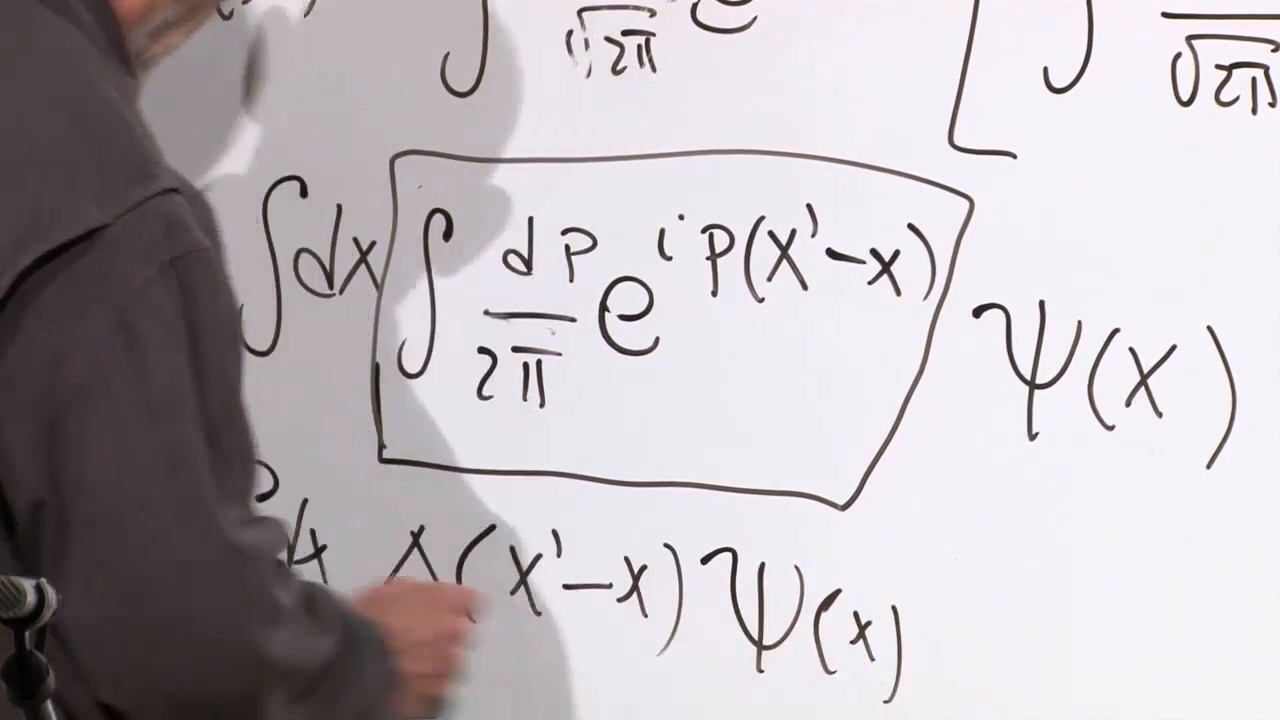
\includegraphics[width=0.88\textwidth]{lecture_09_figure_04.png}
\caption{フーリエ核は2つの変換の合成の内部に孤立しており、そのサンプリング作用によってディラックのデルタとして同定される。}
\lectureframe{00:26:23}
\end{figure}

相互変数の名前を入れ替えると、相補的な恒等式
\begin{equation}
\boxed{
\int_{-\infty}^{\infty}
\frac{dx}{2\pi}\,
e^{ix(p-p')}
=\delta(p-p')
}.
\label{eq:l9-delta-fourier-p}
\end{equation}
が得られる。したがってデルタ関数は平面波の連続的な重ね合わせである。

\begin{classroomqa}
\audiencequestion{指数は一方では\(x'-x\)と書かれ、他方では\(x-x'\)と書かれている。符号の変化は結果を変えるか。}
\lecturerresponse{いいえ。デルタは偶である：\(\delta(u)=\delta(-u)\)。したがって差の符号を反転しても最終的な分布は変わらない。中間の指数関数はその複素共役に変わるが、積分された核は同じデルタである。}
\end{classroomqa}

これらの操作は収束に関する条件を暗黙のうちに省いている。振動積分は絶対収束する通常の積分ではなく超関数であり、積分の順序を変えるには注意が必要である。有限の周期的区間が清浄な正則化を与える：まず離散的なフーリエモードとクロネッカーの直交性を用い、次に区間を無限に大きくする。上の連続体の恒等式はその結果得られる極限である。

\section{直線上の粒子}

古典的には、相空間の一点が状態を指定する：
\begin{equation}
(x,p).
\end{equation}
量子力学は異なる最初の問いを立てる。状態空間を定義する正規直交基底は何か。各実数位置\(x\)に対して、一般化固有ケット\(\ket{x}\)を導入する。一般の状態は次のように展開できる：
\begin{equation}
\ket{\Psi}
=
\int_{-\infty}^{\infty}
dx\,\psi(x)\ket{x},
\qquad
\psi(x)=\braket{x}{\Psi}.
\label{eq:l9-position-expansion}
\end{equation}

\begin{figure}[htbp]
\centering
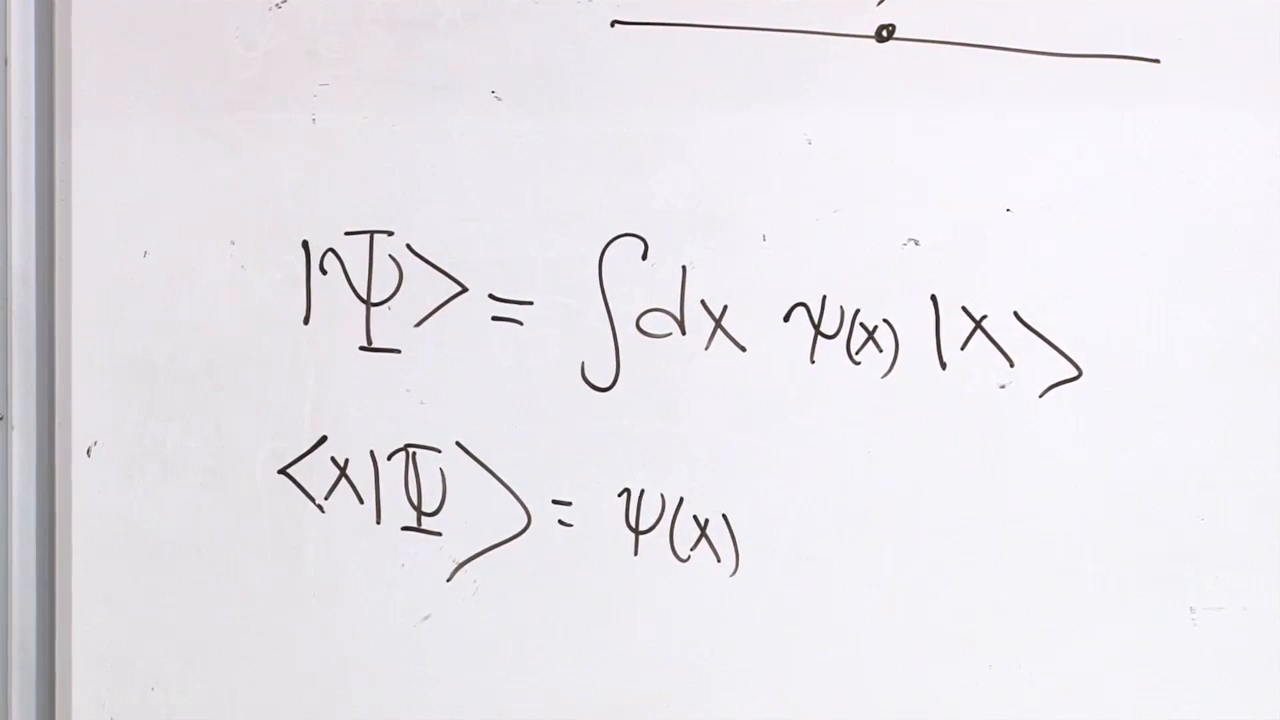
\includegraphics[width=0.88\textwidth]{lecture_09_figure_05.png}
\caption{連続位置基底で展開された一般の状態。その係数は\(\ket{x}\)への射影によって取り出される。}
\lectureframe{00:35:30}
\end{figure}

ボルンの規則は確率密度を
\begin{equation}
\rho(x)=|\psi(x)|^2.
\end{equation}
と与える。有限区間内の確率は
\begin{equation}
P(a<x<b)=\int_a^b|\psi(x)|^2\,dx,
\end{equation}
であり、規格化された物理的状態は
\begin{equation}
\int_{-\infty}^{\infty}|\psi(x)|^2\,dx=1.
\label{eq:l9-position-normalization}
\end{equation}
を満たす。連続的な直交性は
\begin{equation}
\braket{x'}{x}=\delta(x-x').
\label{eq:l9-position-delta}
\end{equation}
で表される。任意の二つの状態について、内積は
\begin{equation}
\braket{\Psi}{\Phi}
=
\int_{-\infty}^{\infty}
dx\,\psi^*(x)\phi(x).
\label{eq:l9-position-inner-product}
\end{equation}
となる。

\begin{figure}[htbp]
\centering
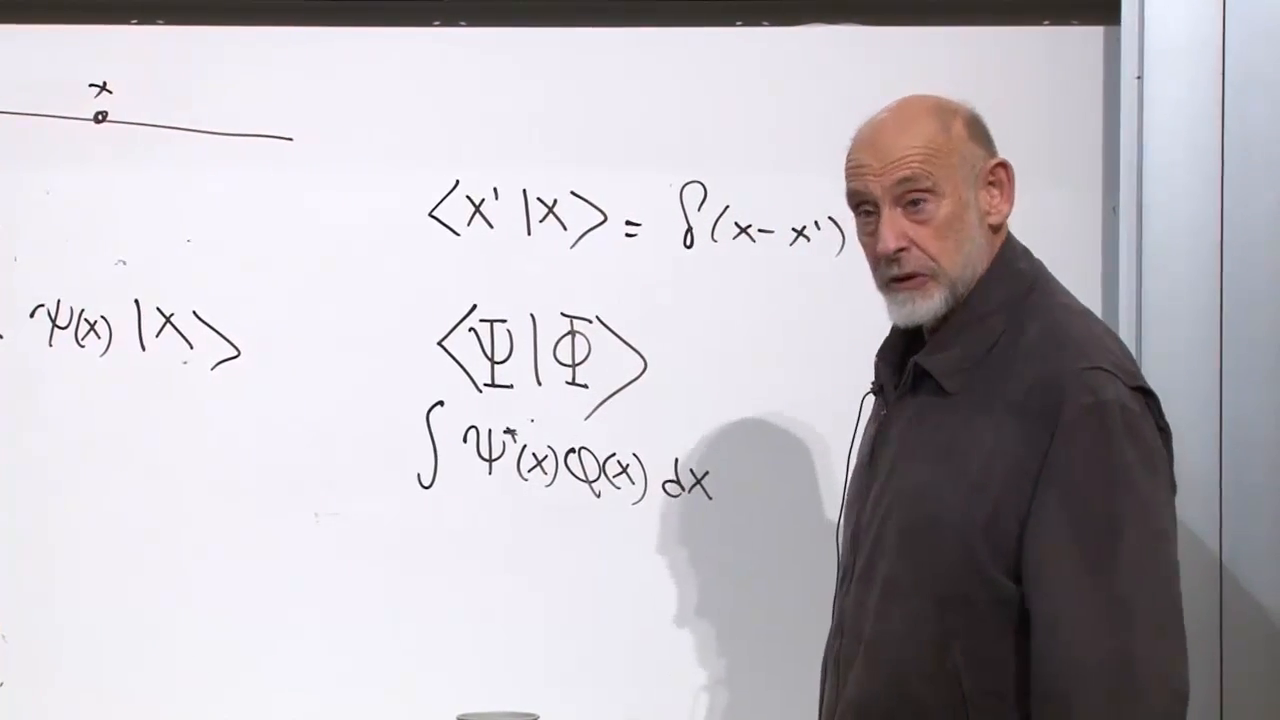
\includegraphics[width=0.88\textwidth]{lecture_09_figure_06.png}
\caption{位置表示で表された連続基底の規格化と波動関数の内積。}
\lectureframe{00:41:20}
\end{figure}

\begin{classroomqa}
\audiencequestion{なぜ位置だけで十分なのか。運動量やほとんど任意の他の変数を加えると冗長になるのか。}
\lecturerresponse{一次元の一粒子では、完全な関数\(\psi(x)\)が状態を指定するので、\(p\)の同時的な確定値は情報として過剰であろう。運動量は、各\(\ket{x}\)に付随する追加のラベルではなく、別の完全な基底を与える。より多くの次元では、両立する情報を混ぜることができる。たとえば\(X\)と\(P_y\)は可換であり、共同基底をラベル付けしてよい。制限は非可換な対に関するものであり、単に記号の数に関するものではない。}
\end{classroomqa}

\begin{classroomqa}
\audiencequestion{運動量も完全な基底を与え、位置を通じて展開できるか。}
\lecturerresponse{はい。運動量基底は完全であり、その係数はフーリエ変換によって位置の係数と関係づけられる。その関係がこの講義の中心的な構成である。}
\end{classroomqa}

\section{位置表示における位置}

抽象的な演算子は状態ベクトルに作用する。基底を選べば、同じ作用は波動関数への具体的な操作になる。位置表示では、位置演算子\(X\)は掛け算として作用する：
\begin{equation}
(X\psi)(x)=x\psi(x).
\label{eq:l9-position-operator}
\end{equation}

\(x_0\)に局在する状態は一般化波動関数\(\delta(x-x_0)\)で表される。\(X\)を作用させると
\begin{align}
X\delta(x-x_0)
&=
x\delta(x-x_0) \notag\\
&=
x_0\delta(x-x_0),
\label{eq:l9-position-eigenfunction}
\end{align}
が得られる。ここで式~\eqref{eq:l9-delta-multiplication}を用いた。したがって\(\delta(x-x_0)\)は固有値\(x_0\)をもつ\(X\)の固有関数である。

\begin{figure}[htbp]
\centering
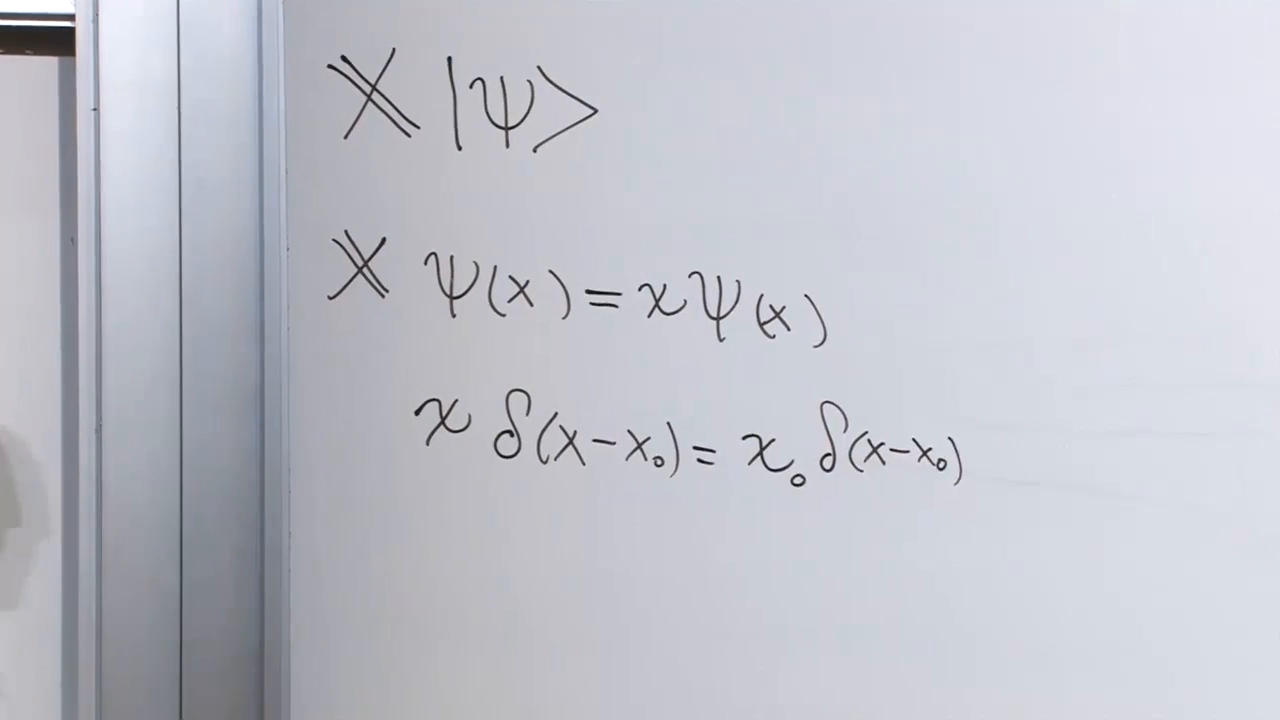
\includegraphics[width=0.88\textwidth]{lecture_09_figure_07.png}
\caption{\(x\)による掛け算は、デルタ局在状態を\(x_0\)倍のそれ自身に変え、それが位置固有関数であることを証明する。}
\lectureframe{00:45:50}
\end{figure}

\(\ket{x_0}\)もそのデルタ関数による代表も、通常の二乗可積分の意味で1に規格化されていない。それはデルタ規格化されている。物理的な局在状態は有限の波束であり、厳密な固有状態は一般化基底ベクトルとしての役割を果たす。

\section{運動量固有関数}

前回の講義で、微分は反エルミートであり、\(-i\)による掛け算がそれをエルミートにすることが分かった。単位を戻して、
\begin{equation}
P=-i\hbar\frac{d}{dx},
\qquad
(P\psi)(x)
=
-i\hbar\frac{d\psi}{dx}.
\label{eq:l9-momentum-operator}
\end{equation}
と定義する。これは適切な定義域上で正当な観測量である。物理的な運動量との同一視は、そのスペクトル、波長、および力学における役割を通じて検証されるであろう。

運動量固有値\(p\)に対して、
\begin{equation}
P\psi_p=p\psi_p,
\end{equation}
または
\begin{equation}
-i\hbar\frac{d\psi_p}{dx}=p\psi_p.
\end{equation}
を解く。解は
\begin{equation}
\psi_p(x)=A e^{ipx/\hbar}.
\label{eq:l9-momentum-eigenfunction}
\end{equation}
である。

\begin{figure}[htbp]
\centering
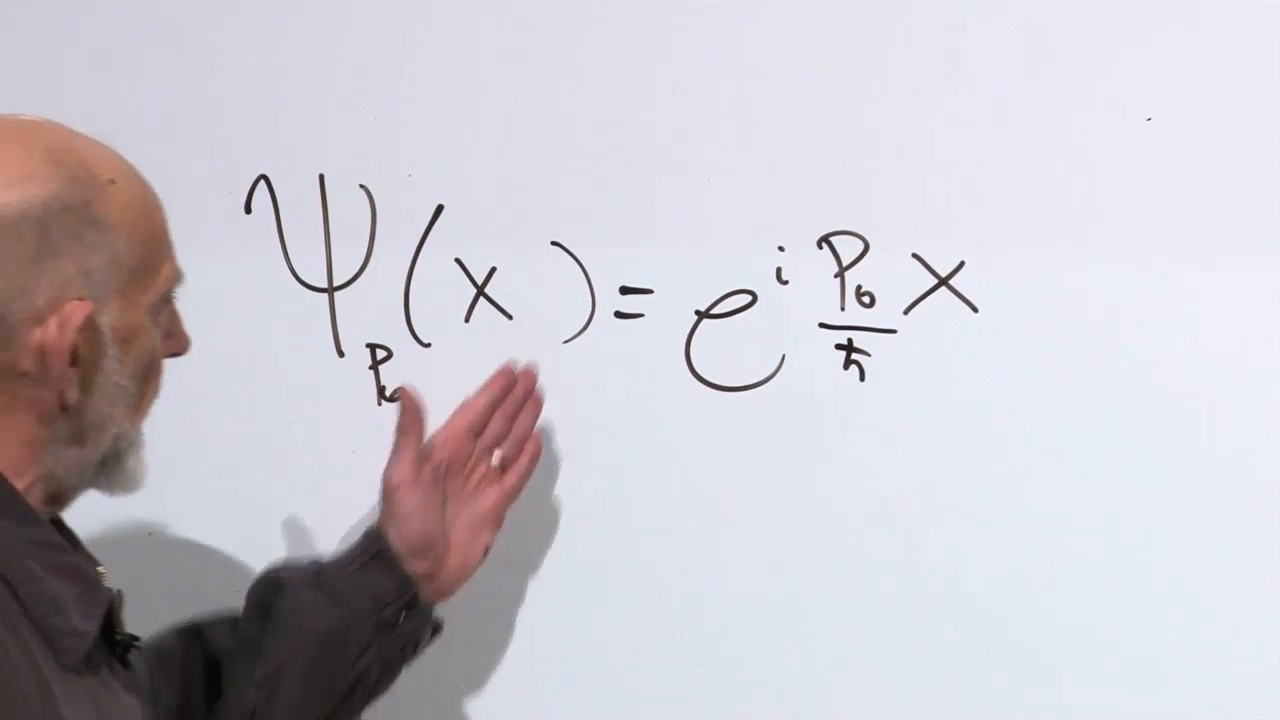
\includegraphics[width=0.88\textwidth]{lecture_09_figure_08.png}
\caption{確定運動量状態の位置空間代表は平面波\(e^{ipx/\hbar}\)である。}
\lectureframe{00:51:45}
\end{figure}

波長\(\lambda\)は位相を\(2\pi\)だけ進める変位である：
\begin{equation}
\frac{p\lambda}{\hbar}=2\pi,
\qquad
\lambda=\frac{2\pi\hbar}{p}.
\label{eq:l9-de-broglie}
\end{equation}
したがって、より大きな運動量はより短い波長に対応する。

デルタ規格化が定数を固定する：
\begin{equation}
\psi_p(x)
=
\frac{1}{\sqrt{2\pi\hbar}}e^{ipx/\hbar}.
\label{eq:l9-normalized-momentum-eigenfunction}
\end{equation}
実際、
\begin{align}
\braket{p'}{p}
&=
\int_{-\infty}^{\infty}
dx\,
\psi_{p'}^*(x)\psi_p(x) \notag\\
&=
\int_{-\infty}^{\infty}
\frac{dx}{2\pi\hbar}
e^{i(p-p')x/\hbar} \notag\\
&=
\delta(p-p').
\label{eq:l9-momentum-normalization}
\end{align}
\(\hbar=1\)とする単位を選んだ後、これらの式は
\begin{equation}
\psi_p(x)=\frac{1}{\sqrt{2\pi}}e^{ipx},
\qquad
\int\frac{dx}{2\pi}e^{i(p-p')x}
=\delta(p-p').
\end{equation}
となる。

\begin{classroomqa}
\audiencequestion{\(p\neq p'\)に対して振動積分が通常の意味で収束しないのに、なぜゼロと宣言できるのか。}
\lecturerresponse{この講義では制御された近道を取る。系を有限の周期的区間に置く。すると許される運動量は離散集合をなし、指数関数は通常の意味で直交し、すべての規格化は有限である。その計算の後に初めて、区間を無限大に飛ばし、クロネッカーデルタをディラックデルタに変える。}
\end{classroomqa}

\begin{classroomqa}
\audiencequestion{同じ収束の問題はデルタ関数のフーリエ変換による導出にも影響するか。}
\lecturerresponse{はい。そこでの積分の交換も同じ理由で形式的であった。有限箱での導出または超関数の言葉が、省略された厳密性を与える。規制された計算が述べられた連続極限をもつので、この近道は許容される。}
\end{classroomqa}

\section{運動量表示}

二つの対象を混同してはならない。式~\eqref{eq:l9-normalized-momentum-eigenfunction}における関数\(\psi_p(x)\)は、特定の固有状態\(\ket{p}\)の位置空間における表示である。これに対して、任意の状態\(\ket{\Psi}\)の運動量空間波動関数は
\begin{equation}
\widetilde{\psi}(p)=\braket{p}{\Psi}.
\label{eq:l9-momentum-wavefunction}
\end{equation}
\(\bra{p}\)と\(\ket{\Psi}\)の位置空間波動関数を代入すると、
\begin{align}
\widetilde{\psi}(p)
&=
\int_{-\infty}^{\infty}
dx\,
\braket{p}{x}\braket{x}{\Psi} \notag\\
&=
\int_{-\infty}^{\infty}
\frac{dx}{\sqrt{2\pi\hbar}}\,
e^{-ipx/\hbar}\psi(x).
\label{eq:l9-position-to-momentum}
\end{align}
これはまさにフーリエ変換である。逆に、
\begin{equation}
\psi(x)
=
\int_{-\infty}^{\infty}
\frac{dp}{\sqrt{2\pi\hbar}}\,
\widetilde{\psi}(p)e^{ipx/\hbar}.
\label{eq:l9-momentum-to-position}
\end{equation}

\begin{figure}[htbp]
\centering
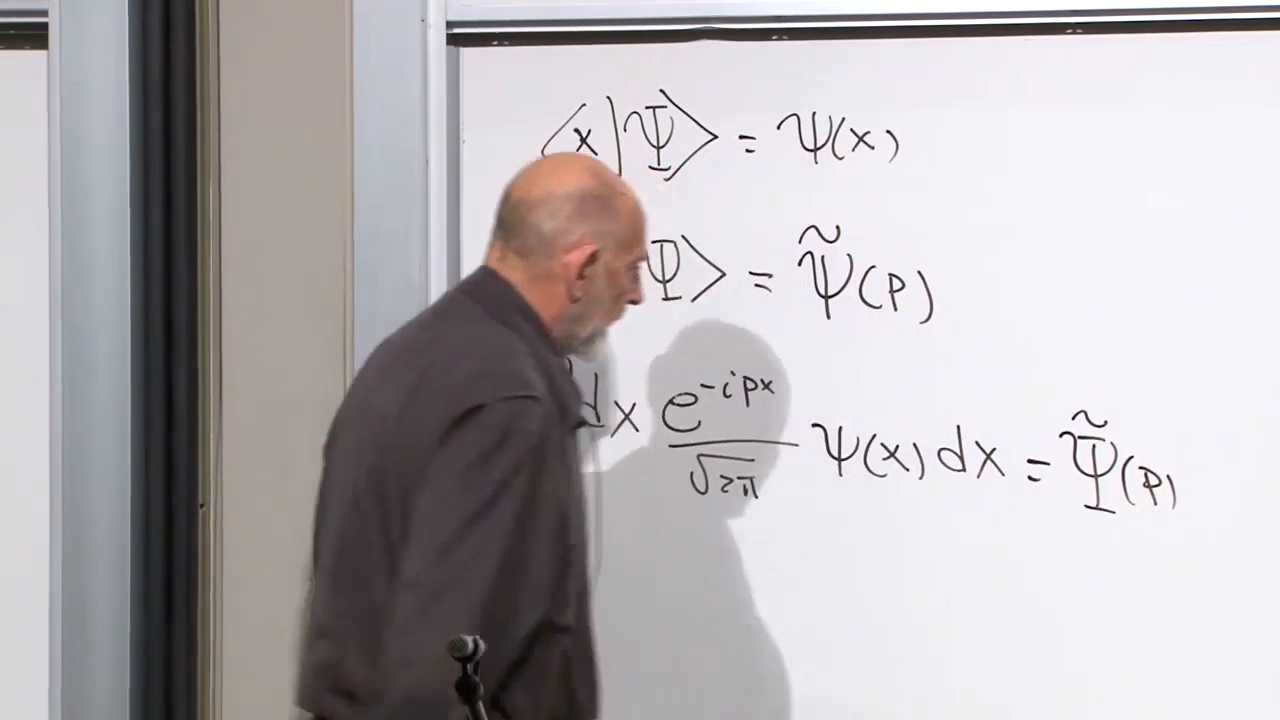
\includegraphics[width=0.88\textwidth]{lecture_09_figure_09.png}
\caption{\(\ket{p}\)への射影は、位置空間波動関数をそのフーリエ変換\(\widetilde{\psi}(p)\)に変える。}
\lectureframe{01:05:50}
\end{figure}

運動量\(p\)を測定する確率密度は
\begin{equation}
\widetilde{\rho}(p)
=
|\widetilde{\psi}(p)|^2,
\qquad
\int_{-\infty}^{\infty}
|\widetilde{\psi}(p)|^2\,dp=1.
\end{equation}
したがって、一つの位置空間波動関数は位置測定と運動量測定の両方を予測するのに十分な情報を含んでいる。運動量の確率を得るには、\(\psi(x)\)をフーリエ変換し、その結果の絶対値を二乗すればよい。

運動量表示では、役割が逆転する：
\begin{equation}
(P\widetilde{\psi})(p)
=
p\widetilde{\psi}(p),
\qquad
(X\widetilde{\psi})(p)
=
i\hbar\frac{d\widetilde{\psi}}{dp}.
\label{eq:l9-operators-in-p}
\end{equation}
\(P=-i\hbar\,d/dx\)との符号の違いは、フーリエ対における符号が逆であることから従う。

\begin{classroomqa}
\audiencequestion{時間は、位置が運動量に共役であるのと同じ仕方でエネルギーに共役な演算子なのか。}
\lecturerresponse{時間は通常、状態の時間発展をラベル付けする外部パラメータとして扱われ、系のヒルベルト空間上の普遍的な自己共役演算子としては扱われない。物理的な時計には確かに観測可能な読みがあり、時計の時間分解能を高めることにはエネルギーの帰結が伴うが、時間とエネルギーの関係は位置と運動量の対よりも慎重な取り扱いを要し、ここでは展開しない。}
\end{classroomqa}

\begin{classroomqa}
\audiencequestion{他にどのような共役対が現れるか。}
\lecturerresponse{角度とそれに対応する角運動量は重要な例を与えるが、角度が周期的であるため大域的な但し書きが付く。場の理論では、場とその正準運動量が共役である。温度と圧力は熱力学的変数であり、正準的な量子の対ではない。一般原理は正準変数とその交換関係によって与えられ、任意の測定可能量の対によって与えられるのではない。}
\end{classroomqa}

\begin{classroomqa}
\audiencequestion{離散的な理論では演算子はケットと波動関数に作用し、波動関数は単に係数を並べたものであった。連続的な理論ではそれは変わったのか。}
\lecturerresponse{いいえ。波動関数は、選ばれた基底における抽象的ケットの座標列である。有限の列に作用する行列と、関数に作用する微分演算子または積分演算子は、同じ抽象的演算の二つの具体的表示である。連続的なラベルは表記を変えるが、論理を変えるものではない。}
\end{classroomqa}

\subsection{フーリエ的事実としての不確定性}

確定した運動量の状態は完全に非局在化している：
\begin{equation}
|\psi_p(x)|^2=\text{constant}.
\end{equation}
その運動量は鋭いが、位置は直線上に一様に広がっている。より一般に、フーリエ対は両方とも狭くなることはできない。\(\widetilde{\psi}(p)\)を運動量の小さな範囲に集中させると、\(\psi(x)\)は大きな領域に広がらざるを得ず、\(\psi(x)\)を局在させるには広い範囲の運動量が必要となる。

この講義ではまだ定量的な不等式
\begin{equation}
\Delta X\,\Delta P\geq\frac{\hbar}{2}.
\end{equation}
を導出していない。現時点での要点は構造的なものである：不確定性原理はすでにフーリエ変換の逆数的な幾何学に組み込まれている。これは、両立しないスピン基底の間を移り変わることの連続版である。

\section{ハミルトニアンが時間発展を生成する}

ハミルトニアン\(H\)はエルミートであり、エネルギーを表し、ユニタリな時間発展を生成する。時間依存のSchr\"odinger方程式は
\begin{equation}
i\hbar\frac{d}{dt}\ket{\Psi(t)}
=
H\ket{\Psi(t)}.
\label{eq:l9-abstract-schrodinger}
\end{equation}
位置表示では、
\begin{equation}
i\hbar\frac{\partial\psi(x,t)}{\partial t}
=
H\psi(x,t),
\label{eq:l9-position-schrodinger}
\end{equation}
ここで右辺は、ハミルトニアンが関数に作用する、選ばれた位置空間表示を意味する。

\subsection{意図的に単純な線形ハミルトニアン}

次のものを取る：
\begin{equation}
H=cP.
\label{eq:l9-linear-hamiltonian}
\end{equation}
これは通常の非相対論的自由粒子のハミルトニアンではない。すべてのステップを直接見ることができるように選ばれたものである。

\begin{figure}[htbp]
\centering
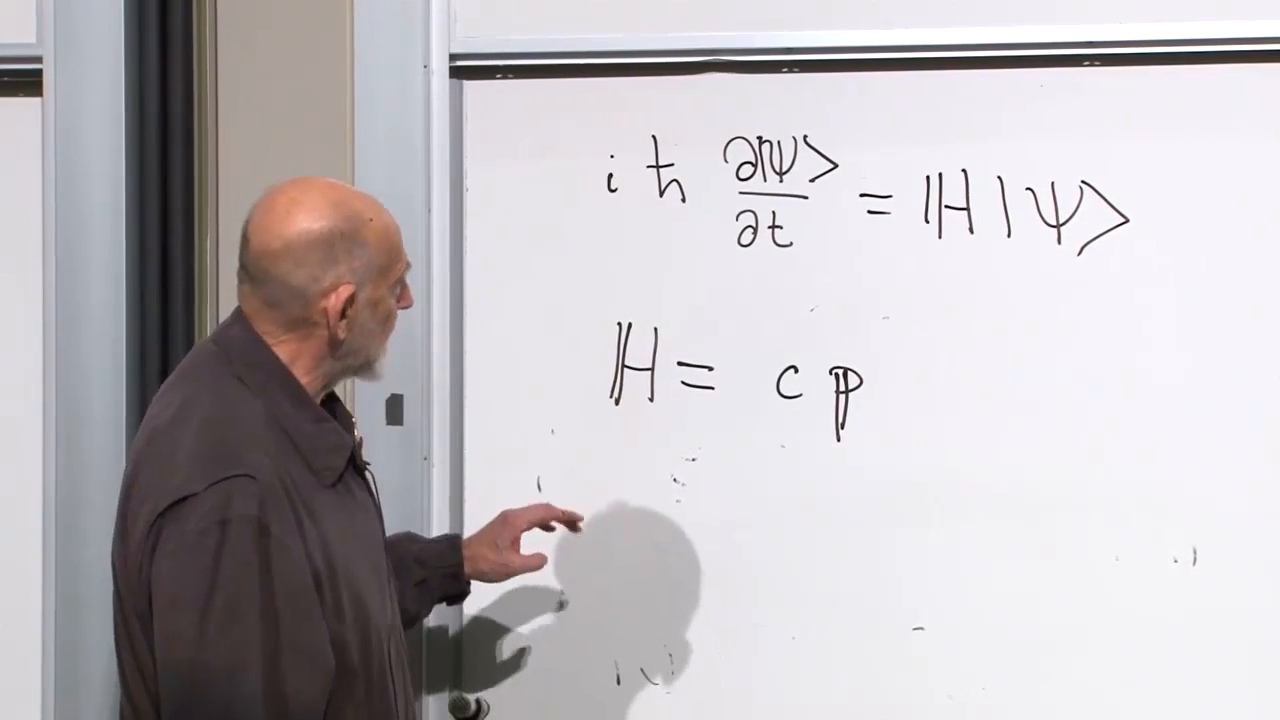
\includegraphics[width=0.88\textwidth]{lecture_09_figure_10.png}
\caption{Schr\"odinger方程式と、粒子の時間発展の最も単純な例として選ばれた線形ハミルトニアン\(H=cP\)。}
\lectureframe{01:17:45}
\end{figure}

\(P=-i\hbar\,\partial_x\)を用いると、
\begin{align}
i\hbar\frac{\partial\psi}{\partial t}
&=
c\left(-i\hbar\frac{\partial}{\partial x}\right)\psi, \notag\\
\frac{\partial\psi}{\partial t}
&=
-c\frac{\partial\psi}{\partial x},
\end{align}
または
\begin{equation}
\frac{\partial\psi}{\partial t}
+c\frac{\partial\psi}{\partial x}=0.
\label{eq:l9-transport-equation}
\end{equation}

\begin{figure}[htbp]
\centering
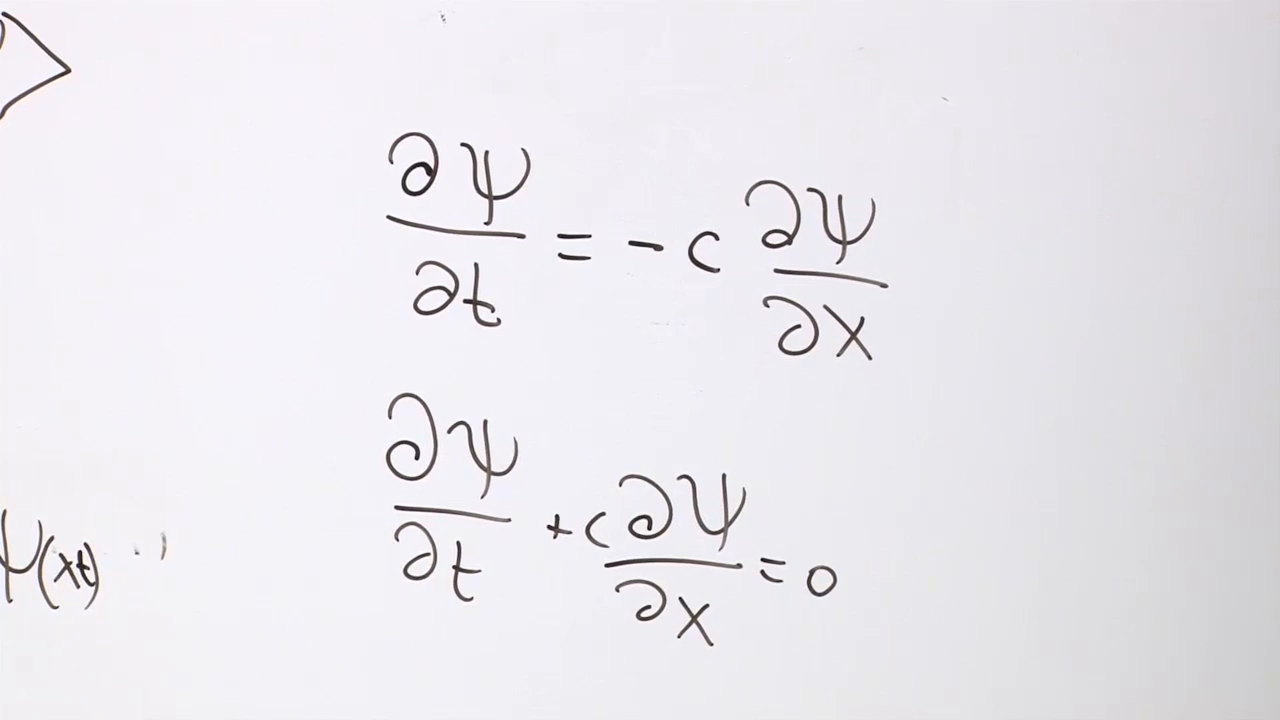
\includegraphics[width=0.88\textwidth]{lecture_09_figure_11.png}
\caption{線形ハミルトニアンはSchr\"odinger方程式を一階の輸送方程式に帰着させる。}
\lectureframe{01:20:05}
\end{figure}

一般解は
\begin{equation}
\psi(x,t)=f(x-ct),
\label{eq:l9-rigid-translation}
\end{equation}
であり、任意の規格化可能な初期プロファイル\(f\)に対して成り立つ。\(t=0\)では、プロファイルは\(f(x)\)である。より後の時刻では、すべての特徴が右へ\(ct\)だけずれている。複素波動関数、その実部と虚部、およびその確率密度はすべてその形を保つ：
\begin{equation}
|\psi(x,t)|^2=|f(x-ct)|^2.
\end{equation}
したがって、
\begin{equation}
\expect{X}_t=\expect{X}_0+ct.
\end{equation}

記号 \(c\) は光速を連想させるために選ばれた。この模型は一次元のカイラルな質量ゼロ励起一つに似ている。許される各成分はすべて一方向に同一の速さで進む。これは完全な光子理論ではない。固定された音速をもつ低エネルギー一次元フォノンも別の類推を与える。\(E=cp\) であるため、\(p\) の両方の符号を許すことは負エネルギーも許すことになり、これが意図的に制限された教育用模型であることを示すもう一つの兆候である。

\begin{classroomqa}
\audiencequestion{もし \(c\) をその粒子の速度に置き換えれば、\(H=cP\) は任意の自由粒子を記述するだろうか。}
\lecturerresponse{いいえ。\(H=cP\) における固定された係数は、すべての運動量成分が同じ速度をもつことを意味する。非相対論的粒子では速度は \(p/m\) であり、したがって運動量に依存する。\(v=p/m\) として \(vP\) を書くことはもはや \(P\) について線形ではなく、二次のハミルトニアンを示唆する。}
\end{classroomqa}

\begin{classroomqa}
\audiencequestion{通常の自由に運動する電子の波動関数は、単に剛体的に平行移動するだけではないのか。}
\lecturerresponse{非常に特別な分散関係だけが、あらゆるプロファイルの剛体的平行移動を生み出す。通常の自由電子の波束は、位相が異なる割合で発展する多くの運動量成分を含む。その中心は動くが、その形は一般に広がる。}
\end{classroomqa}

\subsection{古典的比較}

古典的ハミルトニアン \(H=cp\) に対して、ハミルトンの方程式は次を与える。
\begin{equation}
\dot{x}=\frac{\partial H}{\partial p}=c,
\qquad
\dot{p}=-\frac{\partial H}{\partial x}=0.
\label{eq:l9-linear-hamilton-equations}
\end{equation}

\begin{figure}[htbp]
\centering
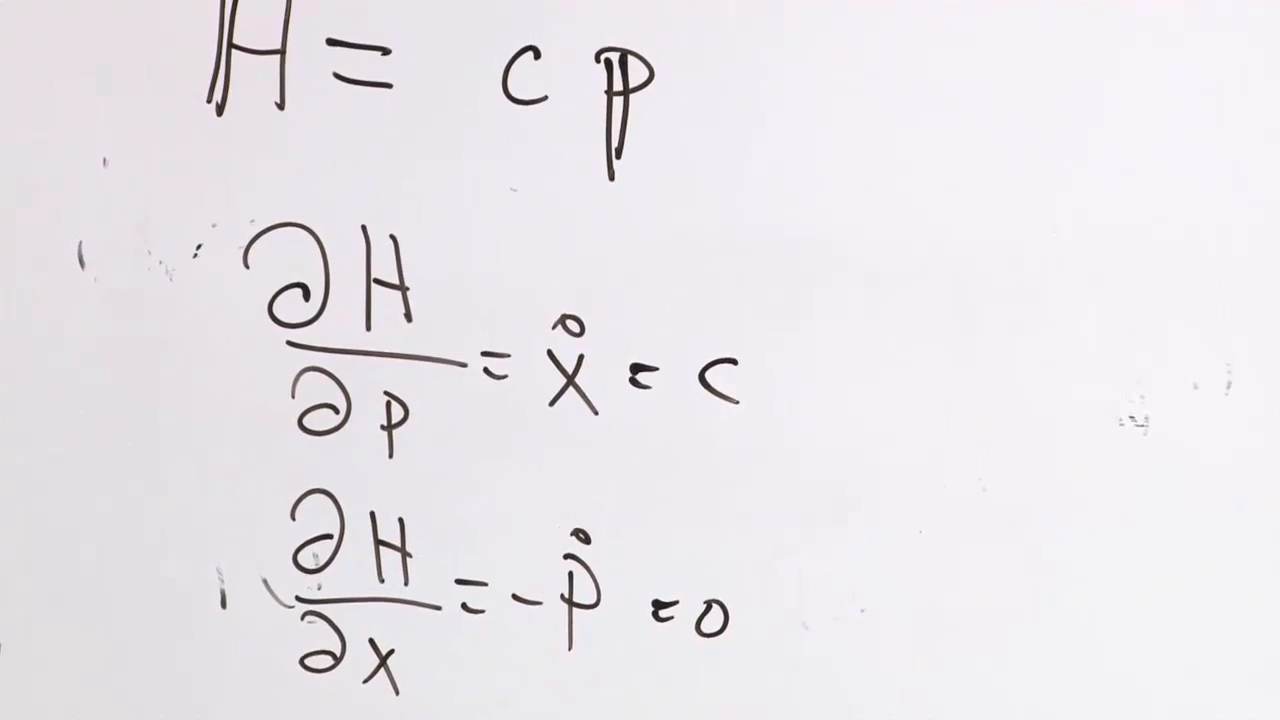
\includegraphics[width=0.88\textwidth]{lecture_09_figure_12.png}
\caption{\(H=cp\) に対するハミルトンの方程式：一定の右向き速度と保存された運動量。}
\lectureframe{01:25:20}
\end{figure}

量子確率分布とその期待値は同じ初等的運動に従う。この一致は、古典的ハミルトニアンから構成された量子発展が適切な意味で古典的方程式を再現すべきであるという最初の具体的な手がかりである。

\section{非相対論的自由粒子}

力を受けない質量 \(m\) の通常の粒子に対して、古典的運動エネルギーは
\begin{equation}
H=\frac{p^2}{2m}.
\end{equation}
である。この二次形式は \(p\) と \(-p\) を対称に扱うので、左向きと右向きの粒子は同じ正のエネルギーをもつ。量子化は \(p\) を演算子 \(P\) に置き換える：
\begin{equation}
H=\frac{P^2}{2m}.
\label{eq:l9-free-hamiltonian}
\end{equation}
\(P=-i\hbar\,\partial_x\) を Schr\"odinger 方程式に代入する：
\begin{align}
i\hbar\frac{\partial\psi}{\partial t}
&=
\frac{1}{2m}
\left(-i\hbar\frac{\partial}{\partial x}\right)^2
\psi \notag\\
&=
-\frac{\hbar^2}{2m}
\frac{\partial^2\psi}{\partial x^2}.
\label{eq:l9-free-schrodinger}
\end{align}

\begin{figure}[htbp]
\centering
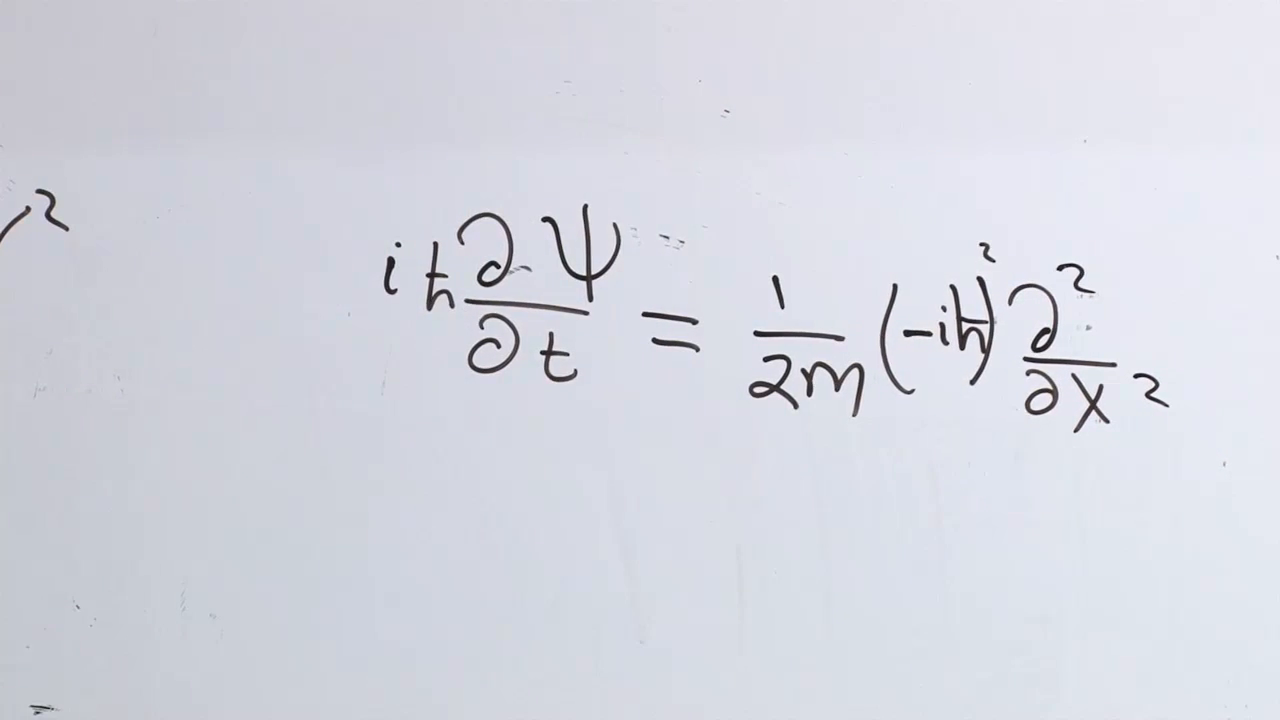
\includegraphics[width=0.88\textwidth]{lecture_09_figure_13.png}
\caption{\(H=P^2/(2m)\) と \(P=-i\hbar\,\partial_x\) から得られる自由粒子 Schr\"odinger 方程式。}
\lectureframe{01:33:50}
\end{figure}

運動量 \(p\) をもつ平面波成分はエネルギー
\begin{equation}
E(p)=\frac{p^2}{2m}.
\end{equation}
をもつ。線形の場合 \(E=cp\) と異なり、この分散関係の傾きは \(p\) に依存する：
\begin{equation}
v_{\mathrm{group}}
=
\frac{dE}{dp}
=
\frac{p}{m}.
\end{equation}
したがって、局在した波束の異なる運動量成分は異なる群速度で進む。それらの相対位相が変化し、成分が分離し、波束は広がる。決定的な対比は、\(H=cP\) があらゆる形を剛体的に輸送するのに対し、\(H=P^2/(2m)\) は分散的な自由粒子運動を生み出すことである。

\section{確立されたこと}

数学的間奏は物理学から切り離されたものではなかった。平面波とディラックのデルタが連続基底の仕組みを構築した。位置演算子は掛け算として作用し、運動量演算子は微分として作用し、運動量固有状態は平面波である。任意の状態をそれらの固有状態に射影すると、その位置波動関数のフーリエ変換が得られる。したがって位置と運動量は一つの状態の競合する表現であり、それらの不確定性はフーリエ対のよく知られた逆幅の関係である。

同じ表現の仕組みが、次にハミルトニアンを微分方程式に変える。運動量の線形関数は剛体的平行移動を生み出し、二次の運動エネルギーは自由粒子 Schr\"odinger 方程式と分散を生み出す。この講義は、測定の基礎から運動の力学へと、その中心的な言語を変えることなく移行した。すなわち状態、基底、エルミート演算子、振幅、そしてユニタリ発展である。
